% !TEX root = calculus.tex

\chapter{LIMIT OF FUNCTION}
{\parindent=0pt
\athr Consider now the concept of the limit of function.

\rdr But we have already covered rather extensively the concept of the limit of a numerical sequence. But a sequence is nothing else but a function defined on a set of natural numbers. Thus, having discussed the limit of sequence, we become acquainted with the limit of function as well. I wonder whether there is any point in a special discussion of the concept of the \emph{limit of function}.

\athr Undoubtedly, a further discussion will be very much to the point. The functions we are concerned with substantially differ from sequences (I have already emphasized this fact) because they are defined over \emph{intervals} and not on sets of natural numbers. This fact makes the concept
of the \emph{limit of function specific}. Note, for example, that every specific convergent sequence has only one limit. It means that the words ``the limit of a given sequence'' are self-explanatory. As for a function defined over an interval, one can speak of an infinite number of ``limits'' because the limit of function is found for each specific point $x = a$ (or, as we say, for $x$ tending to $a$). Thus the phrase ``the limit of a \emph{given} function'' is meaningless because ``the limit of a \emph{given} function must be considered only at each given point $a$''. Besides, this point a should either belong to the domain of the function or coincide with one of the ends of the domain.

\rdr In this case the definition of the limit of function should be very different from that of the limit of sequence.

\athr Certainly, there is a difference.

Note, first of all, that we analyze a function $y = f (x)$, which is defined over a segment, and a point a in this segment (which may coincide with one of its ends when the function is defined over an open or half-open interval).

\rdr Do you mean to say that at the point $x = a$ the function $f (x)$ may not be defined at all?

\athr That is quite correct. Now let us formulate the definition of the limit of function.
\begin{mytheo}{Definition}
A number $b$ is said to be the limit of a function $f (x)$ at $x$ tending to $a$ (the limit at point $a$) if for any positive value of $\varepsilon$ there is a positive value of $\delta$ such that for all $x$ satisfying the conditions $x$ belongs to the domain of the function; $x \neq a$ and 
\begin{equation}%
|x- a| < \delta
\label{lim-delta}
%eq-1
\end{equation}
we have
\begin{equation}%
\left|f(x)- b \right| < \varepsilon
\label{lim-eps}
%eq2
\end{equation}
\end{mytheo}
The standard notation is
\begin{equation*}%
\lim\limits_{x \to a} f (x) = b
\end{equation*}

\rdr The definition of the limit of function is noticeably longer and more complicated than that of the limit of sequence.

\athr Note, first of all, that according to \eqref{lim-delta}, point $x$ should	belong	to	the	interval	 $]a -\delta,	a + \delta[$. Point $x = a$ should be \emph{eliminated} from this interval. The interval $]a -\delta,	a + \delta[$ without point $x = a$ is called a \emph{punctured $\delta$-neighbourhood} of point $a$.

We select an arbitrary positive number $\varepsilon$. For $\varepsilon$ we want to find \emph{another} positive number $\delta$ such that the value of the function at \emph{any} point $x$ from the punctured $
\delta$-neighbourhood of point a must be inside the interval  $]b -\varepsilon,	b + \varepsilon [$ (speaking about \emph{any} point $x$ we imply only the points $x$ in the domain of the function). If there is such $b$ for any $\varepsilon > 0$, $b$ is said to be the limit of the function at point $a$. Otherwise, $b$ is not the limit of the function at point $a$.

\rdr And what does your ``otherwise'' mean in practice?

\athr Assume that the search for $\delta$ has been successful for $n$ diminishing numbers $\varepsilon_{1}, \, \varepsilon_{2}, \, \ldots, \, \varepsilon_{n}$. But then you notice that for a certain number $\varepsilon'$ it is impossible to find the required number $\delta$, i.e. for any value of $\delta$ no matter
how small) there is \emph{always at least one} point $x$ from the punctured $\delta$-neighbourhood of point $a$ at which the value of the function \emph{lies outside} the interval $]b -\varepsilon\,	\, b + \varepsilon' [$.

\rdr But can it happen that we reduce the $\delta$-neighbourhood of point a so much that not a single point $x$, belonging to the domain of the function, remains in the $\delta$-neighbourhood?

\athr Obviously this is impossible. Because the function is defined over an interval, and point $a$ is taken either from this interval or coincides with its end point.

\rdr Everything seems clear. Apparently, in order to root all this firmly in my mind we should discuss the graph of a function.


\athr It is a good idea. Let us analyze, for the sake of convenience, the graph of the function $y = \sqrt{x}$ (\fig{fig-25}). This figure illustrates only two situations. One of them represents the selection of $\varepsilon_{1}$ (see the figure). It is easy to infer that $\delta_{1}$	is the value that we look for: the values of the function at all points $x$ from the $\delta_{1}$-neighbourhood of point a
are inside the interval $]b -\varepsilon_{1} 	\, b + \varepsilon_{1} [$ These values are represented by the portion of the graph between points $A$ and $B$. The second situation represents the selection of $\varepsilon_{2}$.

\begin{figure}[!ht]%[13]{r}{0.5\textwidth}
\centering
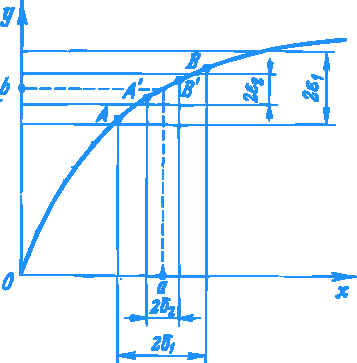
\includegraphics[width=0.6\textwidth]{figures/fig-25.pdf}
\caption{Understanding limit of the function $y = \sqrt{x}$.}
\label{fig-25}
\end{figure}

In this case the number that we seek for is $\delta_{1}$: the values of the function at points $x$ from the $\delta_{2}$-neighbourhood of point a are represented by the portion of the graph between points $A'$ and $B'$.

\rdr Everything you have just described looks so obvious that I see no ``cream'', to use your own words. 

\athr ``The cream'' consists in the following. No matter how small $]b -\varepsilon 	\, b + \varepsilon [$ is, one may always select a $\delta$-neighbourhood for point $a$ such that for all points $x$ in this $\delta$-neighbourhood (all points, with the exception of point $a$ itself and those at which the function is not defined) the values of the function should by all means lie within the indicated interval.

\rdr Could you give an example of a function violating this rule?

\athr For instance, the function $y = \sin \dfrac{1}{x}$ in the
vicinity of point $x = 0$. The graph of the function is plotted in \fig{fig-24}. Obviously, the smaller is $|x|$ the greater is the frequency with which the graph of the function oscillates about the $x$-axis. For an infinitely small $|x|$ the frequency of the oscillations tends to infinity. It is easy to prove that
the function $y = \sin \dfrac{1}{x}$ has no limit at $x = 0$.

\rdr But this function is not defined at zero.

\athr You are right. However, this fact is irrelevant from the viewpoint of the existence (or absence) of the limit of the function at $x = 0$. This function is defined over $]-\infty, 0[$ and $]0, \infty[$. Point $x = 0$ is a common boundary between the intervals over which the function $\sin \dfrac{1}{x}$ is defined. 

But let us return to the concept of the limit. Can we,
for example, state that $b = 0$ is the limit of the function $\sin \dfrac{1}{x}$ at point $x = 0$?

\rdr It seems that I get the point. As long as we
select $\varepsilon > 1$, everything is O.K. But for any $\varepsilon < 1$ it becomes impossible to find a	$\delta$-neighbourhood of	point $x = 0$ such that at all points $x \neq 0$ in this $\delta$-neighbourhood
the values of the function $\sin \dfrac{1}{x}$  are inside the interval
]-8, e]. No matter how \emph{small} the $\delta$-neighbourhood of point $x = 0$ is, it is the segment of \emph{finite} length, so that the graph of our function will oscillate \emph{infinitely many times} and thus will \emph{infinitely many times} go \emph{beyond} $]-\varepsilon,	\, \varepsilon [$.

\athr That's right. Note also that in order to be convinced that a function has no limit, it is sufficient to find a violation even more ``modest''. Namely, it is sufficient that the graph of the function leave the interval $]-\varepsilon,	\, \varepsilon [$ \emph{at least once} for any $\delta$-neighbourhood.

\rdr Apparently, not only $b = 0$ but no other $b \neq 0$ can be the limit of the function $y = \sin \dfrac{1}{x}$ at $x= 0$. Because for any $b \neq 0$ we can use the same arguments as for $b = 0$.

\athr Hence, we have proved that the function $y = \sin \dfrac{1}{x}$ has no limit at point $x=0$.

\rdr The reason for the absence of the limit at $x= 0$ lies in oscillations of the graph of the function. These oscillations become more and more frequent while approaching $x= 0$.

\athr But the reason is not confined only to the infinitely increasing frequency of oscillations of the graph. Another reason is the constancy of the amplitude of oscillations. Let us ``slightly correct'' our function by multiplying
$\sin \dfrac{1}{x}$ by $x$, The graph of the function $y = x \sin \dfrac{1}{x}$ is shown in \fig{fig-26}. Do you think that $b= 0$ is the limit of this function at $x = 0$?

\begin{figure}[!ht]%[13]{r}{0.5\textwidth}
\centering
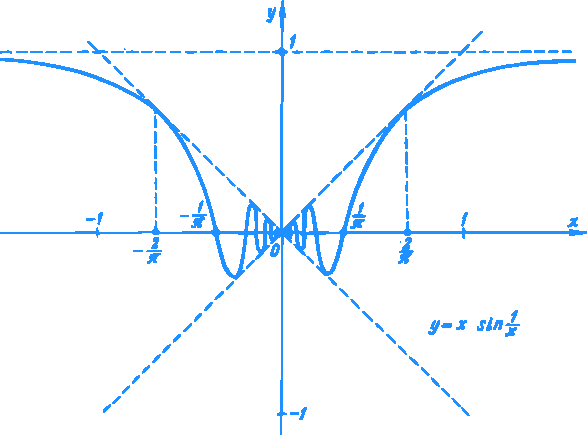
\includegraphics[width=\textwidth]{figures/fig-26.pdf}
\caption{Finding the limit of the function $y = x \sin \dfrac{1}{x}$.}
\label{fig-26}
\end{figure}

\rdr I am at a loss.

\athr I'll answer this question myself. Yes, it is. The proof is within your reach if you use the definition of the limit of function. You are welcome.


\rdr We select an arbitrary $\varepsilon > 0$. We should find $\delta > 0$such that $\left| x \sin \dfrac{1}{x} -0 \right|< \varepsilon$ for all $x$ (excluding $x = 0$) satisfying the condition $|x - 0 |< \delta$. It seems
to me that $\delta$ we look for is $\delta = \varepsilon$.

\athr You are quite right. Because if  $|x| < \delta = \varepsilon$, it becomes evident that $\left| x \sin \dfrac{1}{x}\right| = |x| \left| \sin \dfrac{1}{x} \right| < \varepsilon$.
(since $\left| \sin \dfrac{1}{x} \right| \leqslant 1$). 

\rdr Really, the existence of the limit is proved
without considerable difficulties. 

\athr But, certainly, not always. Consider, for
example, a well-known function $y = \sqrt{x}$ and prove (using the definition of the limit of function) that $b = 1$ is the limit of the function at point $x = 1$.
To begin with, consider the following inequality:
\begin{equation*}%
\left|\sqrt{x} -1  \right| < \varepsilon
\end{equation*}
Try to find a function $g(\varepsilon)$ such that $\left|x - 1 \right|<g(\varepsilon)$
for any $x$ satisfying the condition  $\left|\sqrt{x} - 1 \right|< \varepsilon$

\rdr I understand that $g(\varepsilon)$ is actually the desired $\delta$ 6 corresponding to an arbitrary $\varepsilon$.

\athr Yes, of course. We begin with some transformations. We shall proceed from the inequality:
\begin{equation}%
\left|\sqrt{x} -1 \right| < \varepsilon
\label{ineq-1}
%eq-3
\end{equation}
which can be rewritten in the form:
\begin{equation*}%
(1 - \varepsilon) < \sqrt{x} < (1+ \varepsilon)
\end{equation*}
Since $\sqrt{x} \geqslant 0$, the selection of $\varepsilon < 1$ \emph{a fortiori} (which, of course, does not impair the generality of our proof) allows us to square the last inequalities
\begin{equation*}%
(1 - \varepsilon)^{2} < x < (1+ \varepsilon)^{2}
\end{equation*}
 On removing the parentheses, we obtain
\begin{equation}%
(-2\varepsilon - \varepsilon^{2}) < (x -1) < (2\varepsilon + \varepsilon^{2})
\label{ineq-2}
%eq-4
\end{equation}
Note that inequalities \eqref{ineq-2} are equivalent to \eqref{ineq-1} (provided that $0< \varepsilon < 1$). Now let us proceed from \eqref{ineq-2} to a more exacting inequality:
\begin{equation}%
|x -1| < (2\varepsilon - \varepsilon^{2})
\label{ineq-3}
%eq-5
\end{equation}
(since $0< \varepsilon < 1$, we have $(2\varepsilon - \varepsilon^{2}) > 0$). It is easy to conclude that if \eqref{ineq-3} holds, inequalities \eqref{ineq-2} and, consequently \eqref{ineq-1} will hold all the more. Thus, for an arbitrary $\varepsilon$ within $0< \varepsilon < 1$, it is sufficient to take $\delta = 2 \varepsilon - \varepsilon^{2}$

\rdr What happens if $\varepsilon \gg 1$? 

\athr Then $\delta$ determined for any $\varepsilon < 1$ will be adequate \emph{a fortiori}. 

\rdr Apparently, we may state that
\begin{equation*}%
\lim\limits_{x \to 2} \sqrt{x} = \sqrt{2}, \quad \lim\limits_{x \to 3} \sqrt{x} = \sqrt{3}
\end{equation*}
and, in general, $\lim\limits_{x \to a} \sqrt{x} = \sqrt{a}$.

\athr Yes, that's right. 

\rdr But could we generalize it to
\begin{equation*}%
\lim\limits_{x \to a} f(x) = f(a)
\end{equation*}

\athr Yes, it is often the case. But not always. Because the function $f (x)$ may be undefined at point $a$.
Remember that the limit of the function $y = x \sin \dfrac{1}{x}$ at point
$x = 0$ is zero, but the function itself is not defined at point $x = 0$.

\rdr But perhaps the equality lim f (x) = f (a) x~a
can be considered as valid in all the cases when f (x) is defined at point a?

\athr This may not be correct either. Consider, for example, a function which is called the ``fractional part of $x$''. The standard notation for this function is $\{x\}$. The function is defined on the whole real line. We shall divide the real line into half-intervals $[n, n + 1[$. For $x$ in $[n, n + 1[$ we have $\{x\} = x- n$. The graph of the function $y = \{x\}$ is shown in \fig{fig-27}.

\begin{figure}[!ht]%[13]{r}{0.5\textwidth}
\centering
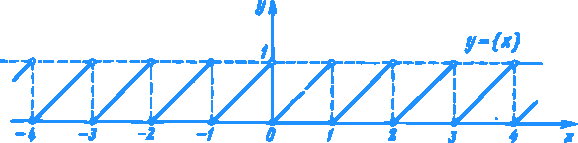
\includegraphics[width=\textwidth]{figures/fig-27.pdf}
\caption{Graph of the function $y = \{x\}$.}
\label{fig-27}
\end{figure}
Take, for example, $x = 1$. It is obvious that $\{x\}$ is defined at point $x = 1 (\{x\} = 0)$. But does the function have the limit at $x = 1$?

\rdr It clearly has no limit. In any $\delta$-neighbourhood of point $x = 1$ there may exist concurrently both the points at which $\{x\}$ assumes values greater than, for example, $\dfrac{2}{3}$, and the points at which $\{x\}$ assumes values less than $\dfrac{1}{3}$.

It means that neither $b= 1$ nor $b=0$ can be the limit of the function at point $x = 1$, if only because it is impossible to find an adequate $\delta$ for  $\varepsilon =\dfrac{1}{3}$.

\athr I see that you have come to be rather fluent in operating with limits of functions. My compliments.

By the way, you have just proved the theorem on the \emph{uniqueness of the limit of function} at a given point.
\begin{mytheo}{Theorem}
A function cannot have two (or more) limits at a given point.
\end{mytheo}
Now let us return to the equality
\begin{equation}%
\lim\limits_{x \to a} f(x) = f(a)
\label{fn-limit}
%eq-06
\end{equation}
You already know that there are situations when $\lim\limits_{x \to a} f(x)$ exists but $f (a)$ does not exist and, vice versa, when $f (a)$
exists but $\lim\limits_{x \to a} f(x)$ does not exist. Finally, a situation is
possible when both $\lim\limits_{x \to a} f(x)$ and $f (a)$ exist, but their 
values are not equal. I'll give you an example: 
\begin{equation*}%
f(x)=
\begin{cases}
 x^{2} & \text{if} \,\, x \neq 0\\
 1 & \text{if} \,\, x=0
 \end{cases}
 \end{equation*}
  The graph of this function is shown in \fig{fig-28}. It is easy
to see that $f(0) = 1$, while $\lim\limits_{x \to a} f(x) =0$.
  
  \begin{figure}[!ht]%[13]{r}{0.5\textwidth}
\centering
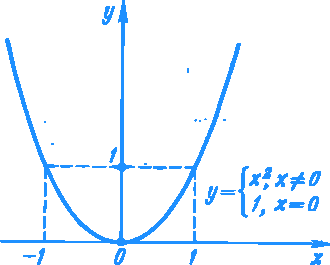
\includegraphics[width=.6\textwidth]{figures/fig-28.pdf}
\caption{Graph of the function $y = f(x)$, such that $f(x) = x^{2}$ for $x \neq 0$ and $f(x) = 1$ for $x = 0$.}
\label{fig-28}
\end{figure}
You must be convinced by now that equality \eqref{fn-limit} is not always valid.

\rdr But presumably, it is often true, isn't it?

\athr Yes, and if it is, the function $f (x)$ is said to be \emph{continuous} at $x = a$.

Thus, we have arrived at a new important concept, namely, that of the \emph{continuity of a function at a point}. Let us give the following definition.
\begin{mytheo}{Definition}
A function $f (x)$ is said to be \emph{continuous at a point} $x = a$ if 
\begin{enumerate}[leftmargin=2cm,label=\protect\circled{\arabic*}]
\item it is defined at $x = a$, 
\item there is the limit of the function at $x = a$, 
\item this limit equals the value of the function at $x = a$;
\end{enumerate}
or, in other words, the function $f (x)$ is called continuous at a point $a$ if
\begin{equation*}%
\lim\limits_{x \to a} f(x) = f(a)
\end{equation*}
\end{mytheo}

I believe that the preceding discussion has brought us so closely to this definition that it needs no additional explanation. I would only like to emphasize that the concept of the continuity of a function is essentially \emph{local}. Similarly to the concept of the limit of function, it is related to a particular point $x$. A function may be either continuous at all points of an interval over which it is defined, or discontinuous at some of its points.

Taking the examples given above, can you single out those functions that are discontinuous at particular points?

\rdr To begin with, I may refer to the function whose graph is plotted in \fig{fig-28}. This function is discontinuous at $x = 0$.

\athr Why?

\rdr Because at this point the function assumes the value $y = 1$, though the limit of the function at this point is apparently zero.

\athr Very good. Can you give other examples?

\rdr The function $y = \{x\}$ (see \fig{fig-27}) is discontinuous at points $x = 0, \,\pm 1, \, \pm2, \, \pm3, \ldots$ The function $y = \sin \dfrac{1}{x}$ (see \fig{fig-24}) is discontinuous at $x = 0$ where it is undefined and, moreover, has no limit. The function whose graph is shown in \fig{fig-14}\textcolor{IndianRed}{($a$)} (see the previous, dialogue) is discontinuous at $x = 2$. The function $y = \tan x$ is discontinuous at points 
\begin{equation*}%
x = \pm \frac{\pi}{2}, \,\, \pm \frac{3\pi}{2}, \,\, \pm \frac{5\pi}{2}, \,\, \pm \frac{7 \pi}{2}
\end{equation*}

\athr That will do. Note that the points at which the continuity of a function is violated are called \emph{discontinuity points}. We say that at these points a function has a discontinuity. In passing through a discontinuity point a graph of a function manifests a singularity. This fact is well illustrated by the examples you have just indicated,

\rdr The discontinuity points in all these examples result in an \emph{interruption of the curve} plotting the function.
One exception is the function  $y = \sin \dfrac{1}{x}$  since it is simply impossible to trace a graph of the function at $x = 0$. 

\athr I may add that neither could you plot the function $y = \tan x$ at its discontinuity points (since you cannot draw a line which ``goes into infinity''). 

\rdr In any case, if a function is continuous everywhere in the domain (has no discontinuity points), its graph is a continuous line: it can be drawn without lifting
the pencil from the paper. 

\athr I agree. I would like to emphasize that the \emph{continuity of a function at a point $x$ guarantees that a very small displacement from this point will result in a very small change in the value of the function}.

Let us turn to \fig{fig-27} which is the graph of the function $y = \{x\}$. Consider, for instance, $x = 0.5$. The function is continuous at this point. It is quite evident that at a very small displacement from the point (either to the left or to the right) the value of the function will also change only a little. Quite a different situation is observed if $x = 1$ (at one of the discontinuity points). At $x = 1$ the function assumes the value $y = 0$. But an infinitesimal shift \emph{to the left} from the point $x = 1$ (take, for example, $x = 0.999$, or $x = 0.9999$, or any other point no matter how close to $x = 1$) will bring a sharp change in the value of the function, from $y= 0$ to $y \approx 1 $.

\rdr Quite clear. I must admit, however, that the local nature of the concept of a continuous function (i.e. the fact that the continuity of a function is always related to a specific point $x$) does not quite conform to the conventional idea of continuity. Because continuity typically implies a process and, consequently, a sort of an interval. It seems that continuity should be related not to a specific moment of time, but to an interval of time.

\athr It is an interesting observation. This local character is a manifestation of one of the specific features of calculus. When analyzing a function at a given point $x$, you used to speak about its value only at this specific point; but calculus operates not only with the value of a function at a point but also with the limit of the function (or its absence) at this point, with the continuity of the function at the point. It means that on the basis of the information about a function at a given point we may construct an image of the \emph{behaviour of the function in the vicinity of this point}. Thus we can predict the behaviour of the function if the point is slightly shifted from $x$.

So far we have made only the first step in this direction. The next step will be the introduction of the concept of a derivative. This will be the subject of discussion in \hyperref[velocity]{Dialogues Eight} and \hyperref[derivative]{Nine}.

\rdr Nevertheless, I would like to note that in the above examples a function was found to be either continuous everywhere over any interval of finite length or discontinuous at a \emph{finite} number of points. In this sense the local nature of the concept of a discontinuity point is evident. The continuity of the function, however, is always observed over a certain interval.

\athr First, the continuity of a function within an interval does not interfere with the local nature of continuity. \emph{A function is continuous over an interval if it is continuous at all points of this interval.}

Second, it is not difficult to construct an example in which the number of discontinuity points over an interval of finite length is \emph{infinitely large}. Let us look, for example, at the following function:
\begin{equation*}%
y =
\begin{cases}
2 & \,\, \text{for} \,\, x= \pm 1, \, \pm \dfrac{1}{2},\, \pm \dfrac{1}{4},\, \pm \dfrac{1}{8},\, \pm \dfrac{1}{16} \ldots \\
x^{2} & \,\, \text{for all the remaining points of the real line, including} \,\, x = 0
\end{cases}
\end{equation*}
The graph of this function is illustrated in \fig{fig-29}. It is easy to conclude that in any $\delta$-neighbourhood of point $x = 0$ the function has an infinite number of discontinuity points.
\begin{figure}[!ht]%[13]{r}{0.5\textwidth}
\centering
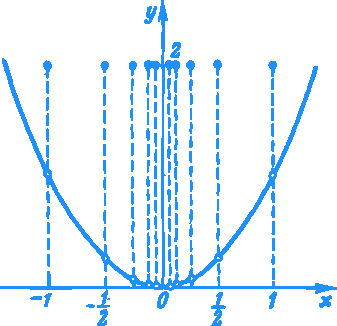
\includegraphics[width=.7\textwidth]{figures/fig-29.pdf}
\caption{Graph of the function $y = f(x)$, such that $f(x) = 2$ for $ x= \pm 1, \, \pm \dfrac{1}{2},\, \pm \dfrac{1}{4},\, \pm \dfrac{1}{8},\, \pm \dfrac{1}{16} \ldots $ and $f(x) = x^{2}$ for all the remaining points of the real line, including $x = 0$.}
\label{fig-29}
\end{figure}

Finally, I can give an example of a function which is discontinuous \emph{at all points of an infinite interval}. This is a function you already know, the Dirichlet function (see the previous dialogue). Being defined on the whole real line, the function has no limit at any point of the real line; consequently, it is discontinuous at each point.

\rdr This is the reason why we in principle cannot plot the Dirichlet function by a graph.

\athr As to the most frequent functions, such as \emph{power, exponential, logarithmic, trigonometric}, and \emph{inverse trigonometric}, they are continuous at all points of the natural domains of the corresponding analytical expressions. The same can be said about composite functions obtained from the above elementary functions. The continuity of all these functions is proved in the more advanced courses of calculus. We limit ourselves to a mere stating of the fact.
}